\documentclass[a4paper,french]{paper}
\usepackage{../../_latex_assets/villemejane_iogs_ceti}

%Informations about this document 
%------------------------------------------
\def\module{Ingénierie Electronique pour le Traitement de l'Information}
\def\moduleAbrege{6N-047-SCI / IéTI}
\def\annee{}

\def\titre{TD 1 / Diodes et sources à LEDs}
\author{Julien VILLEMEJANE}

\subtitle{TD 1}
\institution{LEnsE / Institut d'Optique Graduate School}

\title{\titre}
\begin{document} 
%Beginning First Page. 
%------------------------------------------
\enteteThematiqueObligatoire{}

%Beginning Content. 
%------------------------------------------
\vspace{-1cm}
%%%%%%%%%%%%%%%%%%%
\encadreTDExo{1 - Caractéristique d'une diode}{
On rappelle le symbole et le sens des courants et tensions aux bornes d'une diode :

\begin{center}
	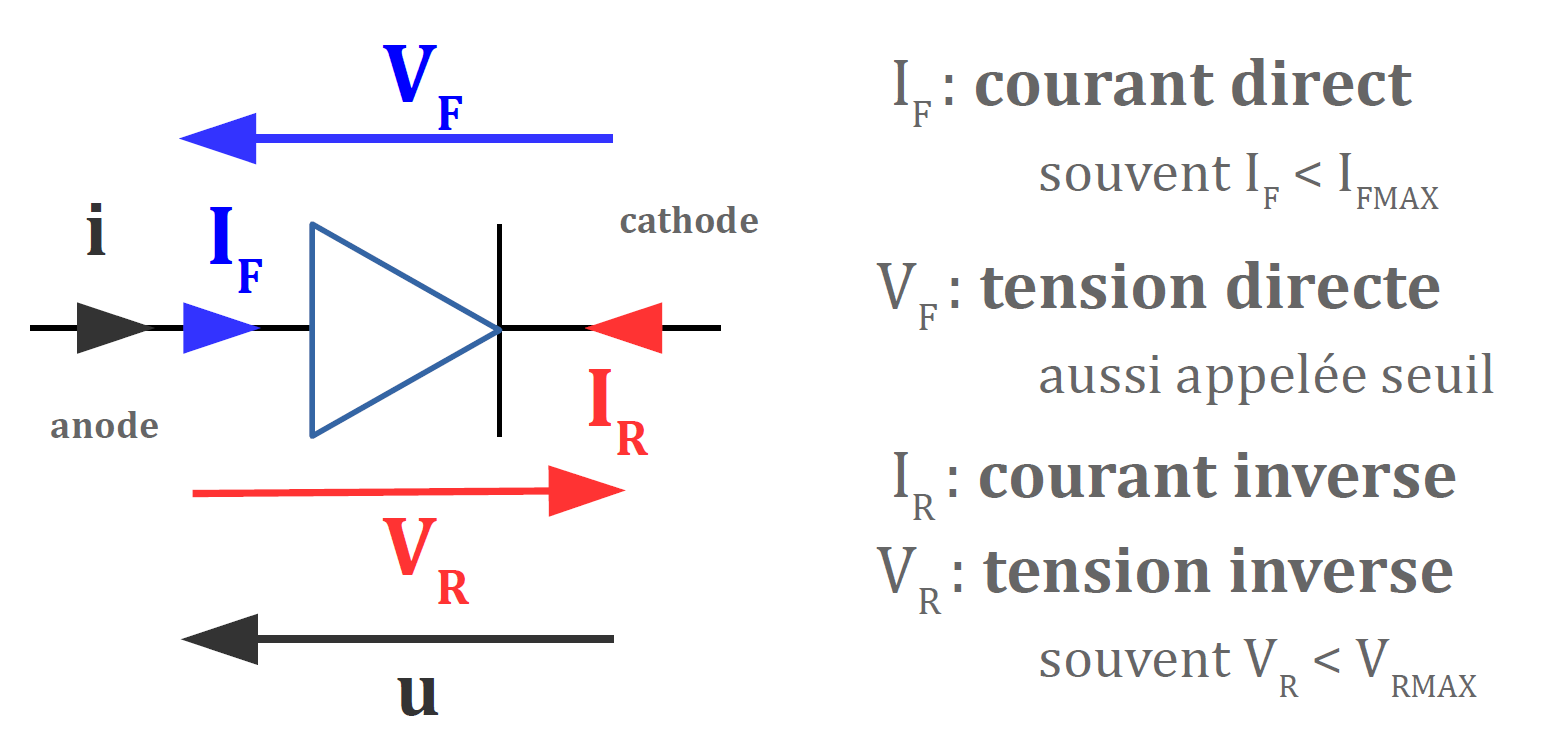
\includegraphics[width=8cm]{images/diodes_000.png}
\end{center}

\medskip
On fournit la documentation technique d'une LED Rouge "classique" (\textit{Kingbright L-53HD}).

\begin{enumerate}
	
	\item Trouvez et relevez la \textbf{caractéristique $I(V)$} de cette LED (allure).
	\item Relevez et commentez l'ensemble des \textbf{paramètres électriques}.
	\item De quel(s) paramètre(s) dépend l'\textbf{intensité lumineuse} émise ?

\end{enumerate}
}

%------------------------------------------
%%%%%%%%%%%%%%%%%%%
\encadreTDExo{2 - Redressement à diodes}{

Soient les circuits suivants :

\begin{center}
	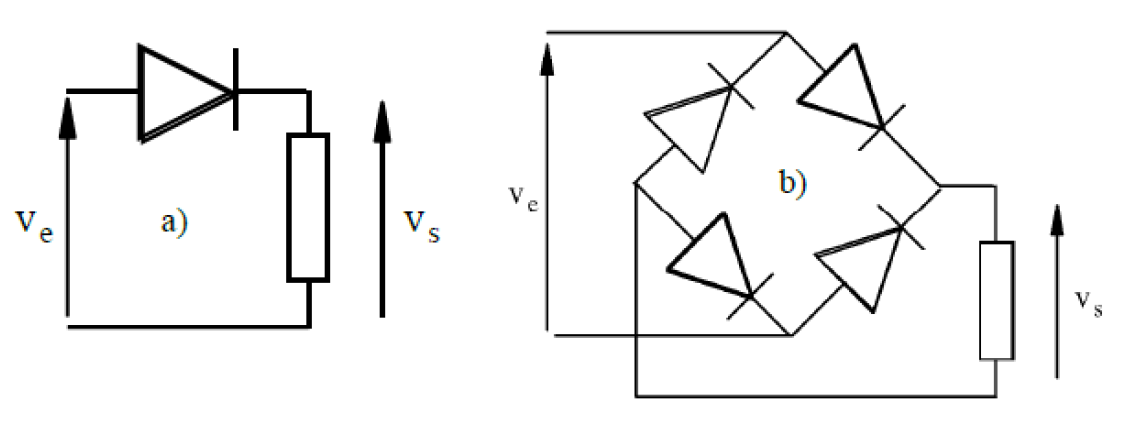
\includegraphics[width=8cm]{images/TD/redresseur_001_a.png}
\end{center}

Donnez l'allure du signal de sortie $V_S(t)$ des circuits a et b suivants pour un signal d'entrée de forme sinusoïdale telle que $V_e(t) = A \cdot sin(\omega{}t)$ dans le cas d'une diode idéale. Puis dans le cas d'une diode avec une tension de seuil $V_d$. On supposera que $A > V_d$.

}


%------------------------------------------
%%%%%%%%%%%%%%%%%%%
\encadreTDExo{3 - Générateurs de signaux}{

On considère à présent les deux montages suivants :

\begin{center}
	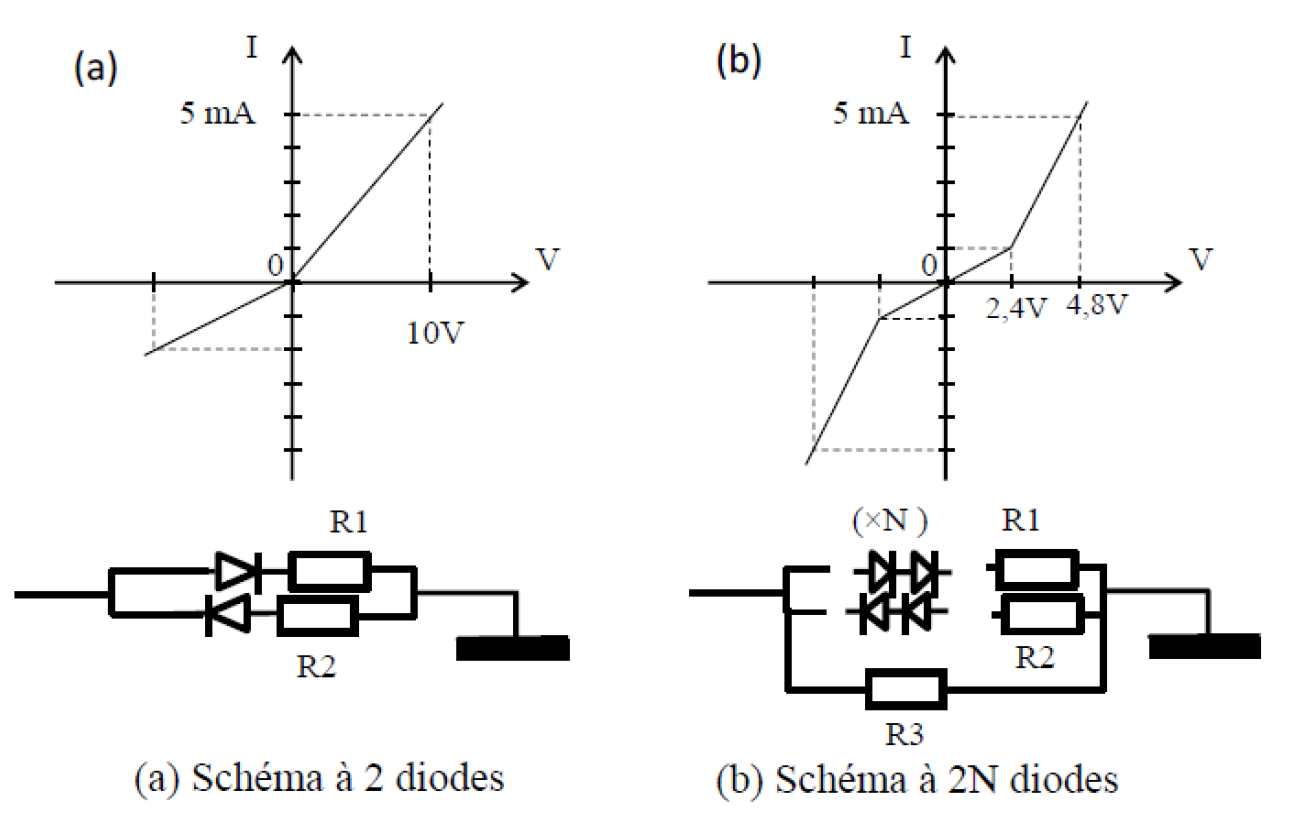
\includegraphics[width=12cm]{images/TD/diodes_002_a.png}
\end{center}

\begin{enumerate}
	\item Dans le cas du montage de la figure (a) et d'utilisation de diodes parfaites et idéales, que doivent valoir $R_1$ et $R_2$ pour obtenir la caractéristique tracée dans le graphe $I(V)$ ?
	\item Dans le cas du montage de la figure (b), les diodes ont pour seuil $0,6\operatorname{V}$. Que doivent valoir $R_1$, $R_2$ et $R_3$ et le nombre de diodes $N$ ($N = 2$ a été dessiné arbitrairement) pour obtenir la caractéristique tracée dans le graphe $I(V)$ ?
\end{enumerate}
}




%------------------------------------------
%%%%%%%%%%%%%%%%%%%
\encadreTDExo{4 - Emetteur à LED}{
On souhaite réaliser un montage émetteur à l'aide de la diode rouge de l'exercice 1. On propose d'étudier le montage suivant :

\begin{center}
	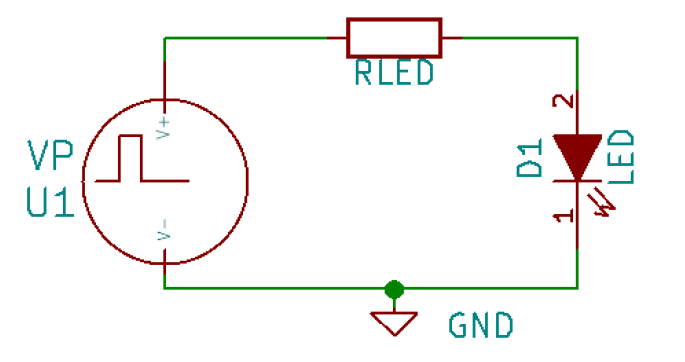
\includegraphics[width=8cm]{images/TD/emetteur_003_a.png}
\end{center}

\begin{enumerate}
	\item Cas 1 : La source de tension $V_P$ est une source continue. Elle délivre une différence de potentiel de $5\operatorname{V}$.
	\begin{enumerate}
		\item Quelle est la valeur maximale du courant que la diode peut supporter dans ces conditions ?
		\item Quelle est la valeur minimale que doit avoir $R_{LED}$ pour respecter cette condition ?
		\item Quel sera alors le courant moyen qui traversera la LED ?
	\end{enumerate}
	
	\item Cas 2 : La source de tension $V_P$ est une source impulsionnelle. Elle délivre des impulsions de $5\operatorname{V}$ de durée $0.1\operatorname{ms}$ avec une fréquence de répétition de $1\operatorname{kHz}$.
	\begin{enumerate}
		\item Quelle est la valeur maximale du courant que la diode peut supporter dans ces conditions ?
		\item Quelle est la valeur minimale que doit avoir $R_{LED}$ pour respecter cette condition ?
		\item Quel sera alors le courant moyen qui traversera la LED ?
	\end{enumerate}

	\bigskip
	
	On s'intéresse maintenant à une LED infrarouge (IR) de type SFH415 (documentation fournie en annexe). 

	\item Cas 2bis : La source de tension $V_P$ est une source impulsionnelle. Elle délivre des impulsions de $5\operatorname{V}$ de durée $0.1\operatorname{ms}$ avec une fréquence de répétition de $1\operatorname{kHz}$.
	\begin{enumerate}
		\item Quelle est la valeur maximale du courant que la diode peut supporter dans ces conditions ?
		\item Quelle est la valeur minimale que doit avoir $R_{LED}$ pour respecter cette condition ?
		\item Quel sera alors le courant moyen qui traversera la LED ?
		\item Quelle sera la puissance dissipée dans la résistance $R_{LED}$ ?
	\end{enumerate}
\end{enumerate}
}

\includepdf[pages=2-3]{docs/doc_LEDRouge.pdf}

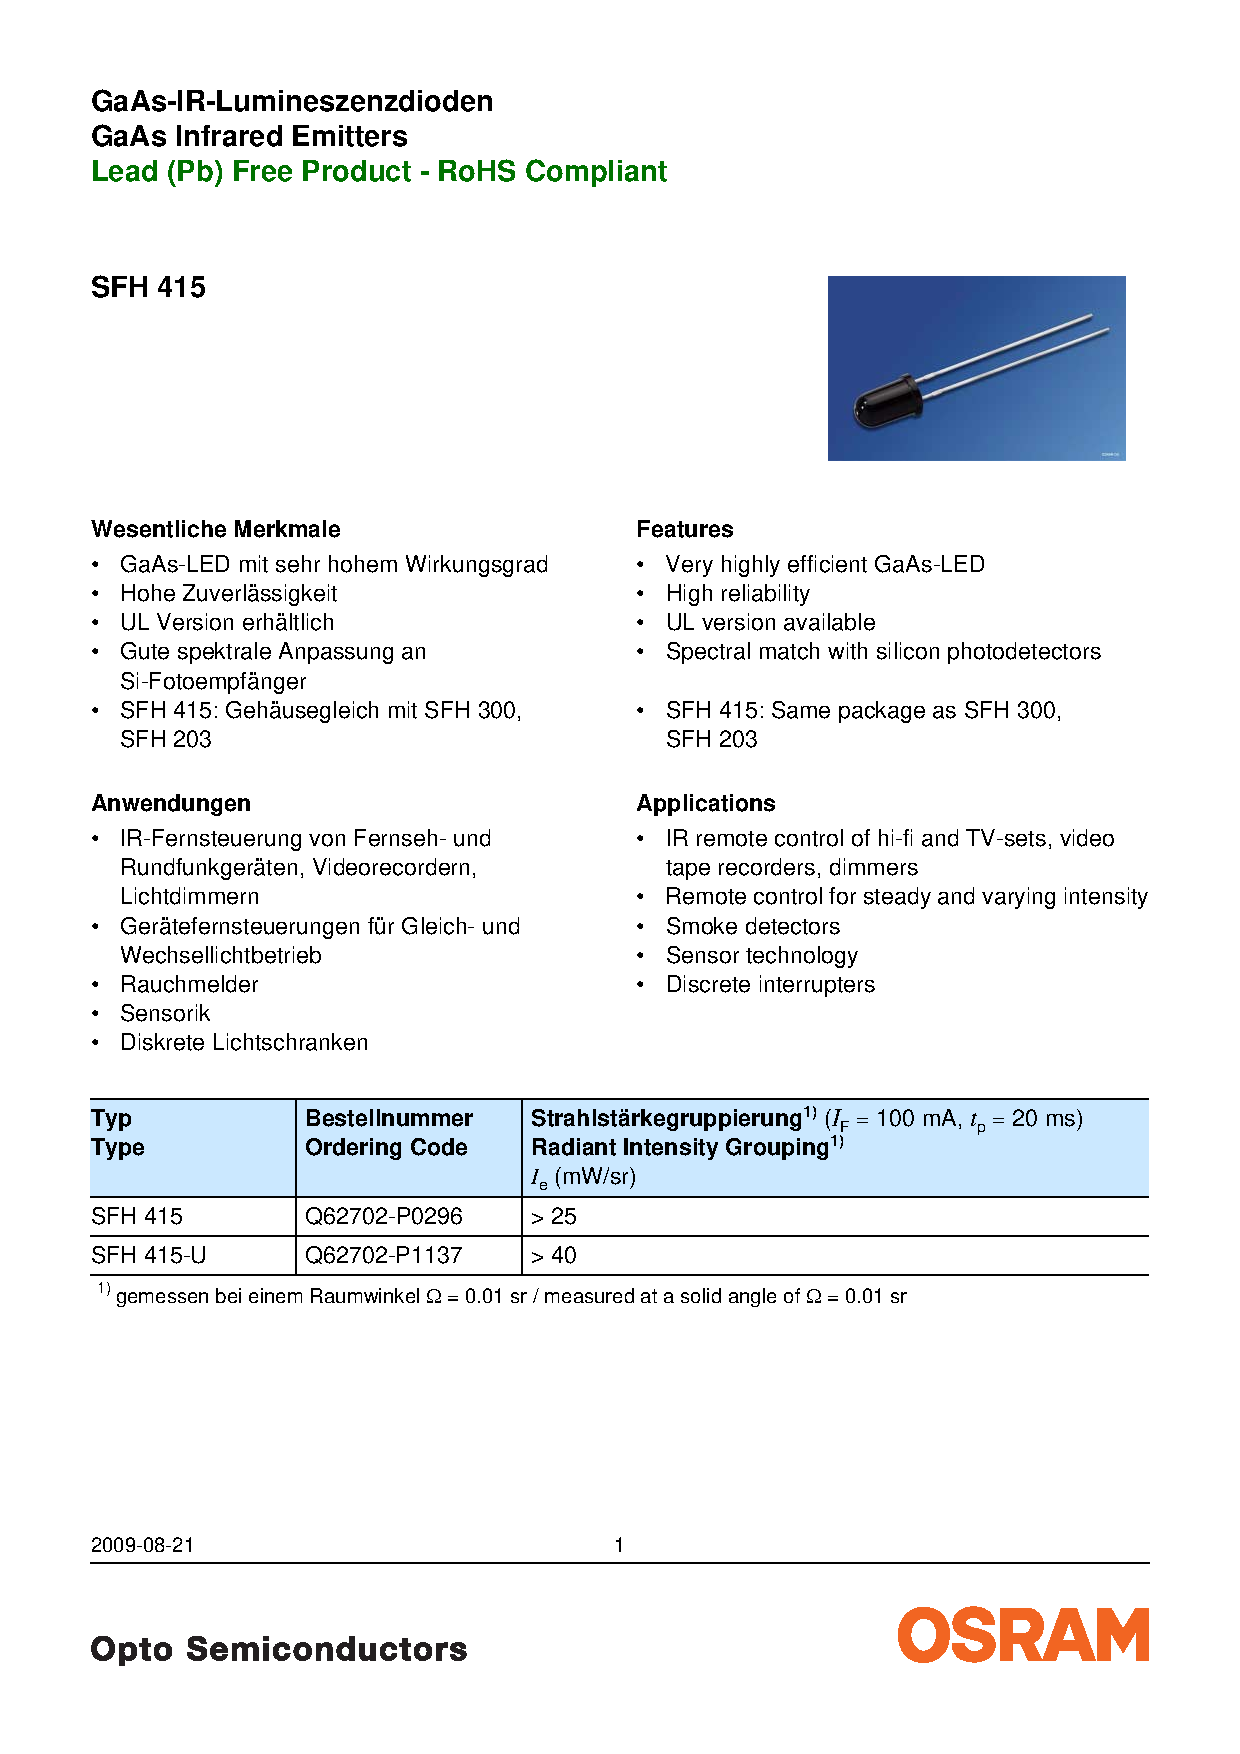
\includepdf[pages={1-3,5}]{docs/doc_IR_SFH415.pdf}

\end {document}